% Created 2014-04-03 Thu 22:07
\documentclass[table,smaller]{beamer}
\usepackage[utf8]{inputenc}
\usepackage[T1]{fontenc}
\usepackage{fixltx2e}
\usepackage{graphicx}
\usepackage{longtable}
\usepackage{float}
\usepackage{wrapfig}
\usepackage{rotating}
\usepackage[normalem]{ulem}
\usepackage{amsmath}
\usepackage{textcomp}
\usepackage{marvosym}
\usepackage{wasysym}
\usepackage{amssymb}
\usepackage{hyperref}
\tolerance=1000
\usepackage{tikz}
\usepackage{minted}
\usepackage{fancyvrb}
\usemintedstyle{perldoc}
\definecolor{lightgray}{gray}{0.96}
\setlength{\tabcolsep}{1ex}
\institute{Harvard MIT Data Center}
\usetheme{Warsaw}
\useoutertheme{infolines}
\setbeamercolor{block body}{bg=lightgray}
\titlegraphic{
\includegraphics[width=.75\textwidth]{images/IQSSNewLogo.pdf}}
\setbeamersize{text margin left=2em,text margin right=2em}
\AtBeginSection[]{\begin{frame}<beamer>\frametitle{Topic}\tableofcontents[currentsection]\end{frame}}
\usetheme{default}
\author{}
\date{}
\title{Regression in Stata}
\hypersetup{
  pdfkeywords={},
  pdfsubject={},
  pdfcreator={Emacs 24.3.1 (Org mode 8.2.5h)}}
\begin{document}

\maketitle
\begin{frame}{Outline}
\tableofcontents
\end{frame}


\section{Introduction}
\label{sec-1}
\rowcolors{1}{blue!15}{blue!3}
\definecolor{bg}{rgb}{0.95,0.95,0.95}
\definecolor{cbg}{cmyk}{0,0,.1,0}

\begin{frame}[fragile,label=sec-1-1]{Download workshop materials}
 \begin{itemize}
\item Download materials from \url{http://j.mp/stata-stats}
\item Extract materials from the \texttt{StataStatistics.zip} file
\item Launch Stata and open the \texttt{StataStatistics.do} file
\end{itemize}
\end{frame}

\begin{frame}[label=sec-1-2]{Organization}
\begin{itemize}
\item Please feel free to ask questions at any point if they are relevant to the current topic (or if you are lost!)
\item There will be a Q\&A after class for more specific, personalized questions
\item Collaboration with your neighbors is encouraged
\item If you are using a laptop, you will need to adjust paths accordingly
\item Make comments in your Do-file rather than on hand-outs
\item Save on flash drive or email to yourself
\end{itemize}
\end{frame}
\begin{frame}[label=sec-1-3]{Today's Dataset}
\begin{itemize}
\item We have data on a variety of variables for all 50 states
\item Population, density, energy use, voting tendencies, graduation rates, income, etc.
\item We're going to be predicting SAT scores
\item Univariate Regression: SAT scores and Education Expenditures
\item Does the amount of money spent on education affect the mean SAT score in a state?
\item Dependent variable: csat
\item Independent variable: expense
\end{itemize}
\end{frame}
\begin{frame}[fragile,label=sec-1-4]{Opening Files in Stata}
 \begin{itemize}
\item Look at bottom left hand corner of Stata screen
\begin{itemize}
\item This is the directory Stata is currently reading from
\end{itemize}
\item Files are located in the StataStatistics folder on the Desktop
\item Start by telling Stata where to look for these
\end{itemize}

\begin{minted}[fontsize=\footnotesize]{c}
* change directory
cd "~/StataStatistics"
\end{minted}


\begin{itemize}
\item Use dir to see what is in the directory:
\end{itemize}


\begin{minted}[fontsize=\footnotesize]{c}
dir
\end{minted}


\vspace{-.5em}
\begin{columns}
\column{.95\linewidth}
\begin{block}{}
\begin{minted}[linenos=false, fontsize=\tiny]{c}
-rw-r--r--  1 izahn  staff    3935 Jan 23 18:05 Regression in Stata.do
-rw-r--r--  1 izahn  staff    7816 Apr  5 17:14 StataStatistics.txt
-rw-r--r--  1 izahn  staff   13630 Jan 23 18:03 states.dta
\end{minted}
\end{block}
\end{columns}
\vspace{.5em}

\begin{itemize}
\item Load the data
\end{itemize}

\begin{minted}[fontsize=\footnotesize]{c}
* use the states data set
use states.dta
\end{minted}
\end{frame}

\begin{frame}[label=sec-1-5]{Steps for Running Regression}
\begin{enumerate}
\item Examine descriptive statistics
\item Look at relationship graphically and test correlation(s)
\item Run and interpret regression
\item Test regression assumptions
\end{enumerate}
\end{frame}

\section{Univariate regression}
\label{sec-2}

\begin{frame}[fragile,label=sec-2-1]{Univariate Regression: Preliminaries}
 \begin{itemize}
\item We want to predict csat scores from expense
\item First, let's look at some descriptives
\end{itemize}

\begin{minted}[fontsize=\footnotesize]{c}
* generate summary statistics for csat and expense
sum csat expense
\end{minted}

\vspace{-.5em}
\begin{columns}
\column{.95\linewidth}
\begin{block}{}
\begin{minted}[linenos=false, fontsize=\tiny]{c}
    Variable |       Obs        Mean    Std. Dev.       Min        Max
-------------+--------------------------------------------------------
        csat |        51     944.098    66.93497        832       1093
     expense |        51    5235.961    1401.155       2960       9259
\end{minted}
\end{block}
\end{columns}
\vspace{.5em}
\end{frame}

\begin{frame}[fragile,label=sec-2-2]{Univariate Regression Preliminaries}
 \begin{itemize}
\item We want to predict csat scores from expense
\item First, let's look at some descriptives
\end{itemize}

\begin{minted}[fontsize=\footnotesize]{c}
* look at codebok
codebook csat expense
\end{minted}

\vspace{-.5em}
\begin{columns}
\column{.95\linewidth}
\begin{block}{}
\begin{minted}[linenos=false, fontsize=\tiny]{c}
-------------------------------------------------------------------------------
csat                                                   Mean composite SAT score
-------------------------------------------------------------------------------
                  type:  numeric (int)
                 range:  [832,1093]                   units:  1
         unique values:  45                       missing .:  0/51
                  mean:   944.098
              std. dev:    66.935
           percentiles:        10%       25%       50%       75%       90%
                               874       886       926       997      1024
-------------------------------------------------------------------------------
expense                                         Per pupil expenditures prim&sec
-------------------------------------------------------------------------------
                  type:  numeric (int)
                 range:  [2960,9259]                  units:  1
         unique values:  51                       missing .:  0/51
                  mean:   5235.96
              std. dev:   1401.16
           percentiles:        10%       25%       50%       75%       90%
                              3782      4351      5000      5865      6738
\end{minted}
\end{block}
\end{columns}
\vspace{.5em}
\end{frame}

\begin{frame}[fragile,label=sec-2-3]{Univariate Regression Preliminaries}
 \begin{itemize}
\item Next, view relationship graphically
\item Scatterplots work well for univariate relationships
\end{itemize}



\begin{minted}[fontsize=\footnotesize]{c}
* graph expense by csat
twoway scatter expense csat
\end{minted}


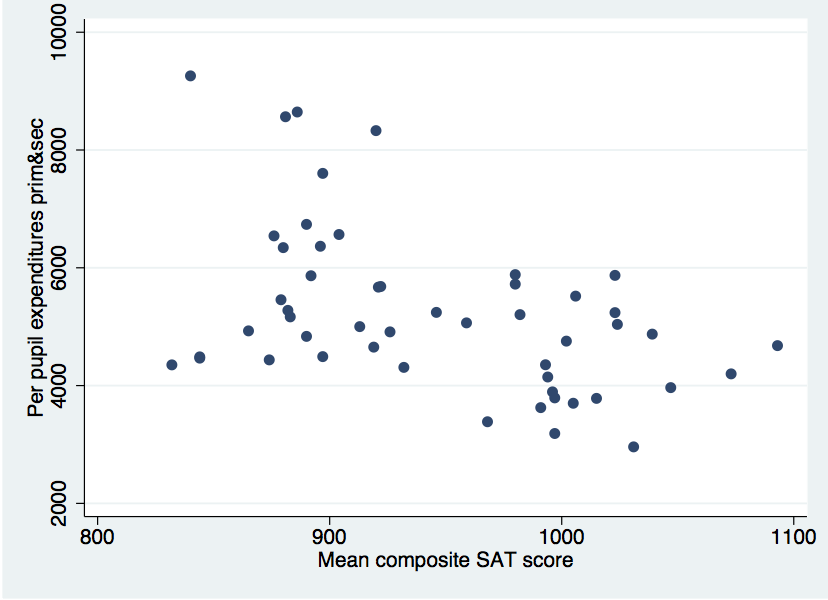
\includegraphics[width=.6\textwidth]{images/scatter1.png}
\end{frame}


\begin{frame}[fragile,label=sec-2-4]{Univariate Regression Preliminaries}
 \begin{itemize}
\item Next look at the correlation matrix
\end{itemize}

\begin{minted}[fontsize=\footnotesize]{c}
* correlate csat and expense
pwcorr csat expense, star(.05)
\end{minted}

\vspace{-.5em}
\begin{columns}
\column{.95\linewidth}
\begin{block}{}
\begin{minted}[linenos=false, fontsize=\tiny]{c}
             |     csat  expense
-------------+------------------
        csat |   1.0000 
     expense |  -0.4663*  1.0000
\end{minted}
\end{block}
\end{columns}
\vspace{.5em}



\begin{itemize}
\item Not very interesting with only one predictor
\end{itemize}
\end{frame}
\begin{frame}[fragile,label=sec-2-5]{Univariate Regression: SAT scores and Education Expenditures}
 \begin{minted}[fontsize=\footnotesize]{c}
regress csat expense
\end{minted}

\vspace{-.5em}
\begin{columns}
\column{.95\linewidth}
\begin{block}{}
\begin{minted}[linenos=false, fontsize=\tiny]{c}
   Source |       SS       df       MS              Number of obs =      51
----------+------------------------------           F(  1,    49) =   13.61
    Model |  48708.3001     1  48708.3001           Prob > F      =  0.0006
 Residual |   175306.21    49  3577.67775           R-squared     =  0.2174
----------+------------------------------           Adj R-squared =  0.2015
    Total |   224014.51    50   4480.2902           Root MSE      =  59.814

---------------------------------------------------------------------------
     csat |      Coef.   Std. Err.      t    P>|t|     [95% Conf. Interval]
----------+----------------------------------------------------------------
  expense |  -.0222756   .0060371    -3.69   0.001    -.0344077   -.0101436
    _cons |   1060.732    32.7009    32.44   0.000     995.0175    1126.447
---------------------------------------------------------------------------
\end{minted}
\end{block}
\end{columns}
\vspace{.5em}
\end{frame}


\begin{frame}[label=sec-2-6]{Linear Regression Assumptions}
\begin{itemize}
\item Assumption 1: Normal Distribution
\item The errors of regression equation are normally distributed
\item Assumption 2: Homoscedasticity (The variance around the regression line is the same for all values of the predictor variable)
\item Assumption 3: Errors are independent
\item Assumption 4: Relationships are linear
\end{itemize}
\end{frame}
\begin{frame}[label=sec-2-7]{Homoscedasticity}
{\center
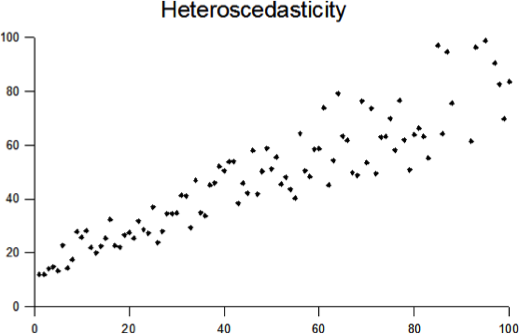
\includegraphics[width=.5\textwidth]{images/heteroscedasticity.png}

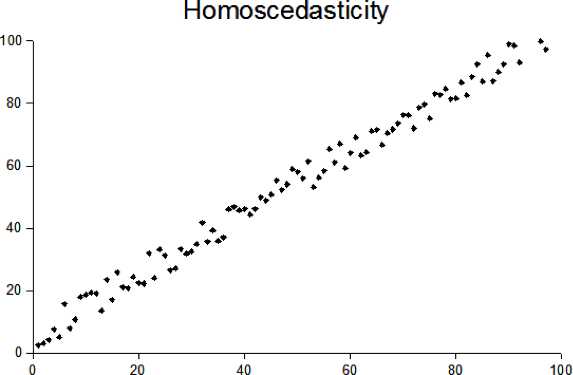
\includegraphics[width=.5\textwidth]{images/homscedasticity.png}

}
\end{frame}
\begin{frame}[fragile,label=sec-2-8]{Testing Assumptions: Normality}
 \begin{itemize}
\item A simple histogram of the residuals can be informative
\end{itemize}

\begin{minted}[fontsize=\footnotesize]{c}
* graph the residual values of csat
predict resid, residual
histogram resid, normal
\end{minted}

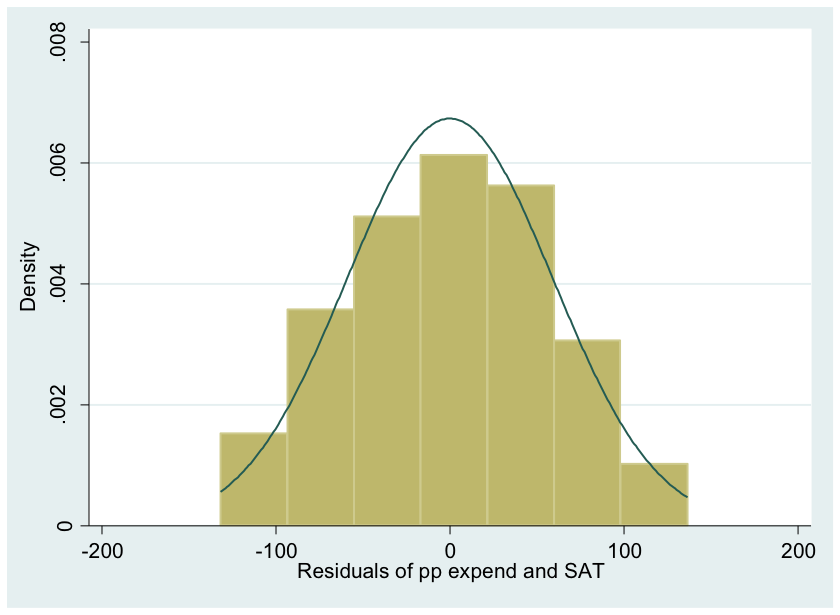
\includegraphics[width=.6\textwidth]{images/normalHist1.png}
\end{frame}

\begin{frame}[fragile,label=sec-2-9]{Testing Assumptions: Homoscedasticity}
 \begin{minted}[fontsize=\footnotesize]{c}
rvfplot
\end{minted}


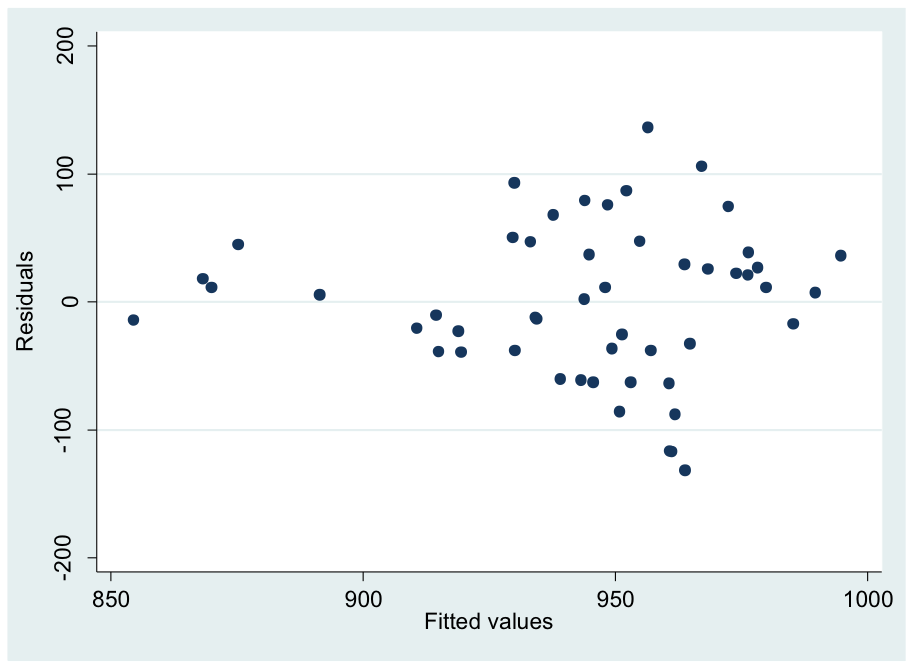
\includegraphics[width=.6\textwidth]{images/fittedResidual1.png}
\end{frame}


\section{Multiple regression}
\label{sec-3}

\begin{frame}[label=sec-3-1]{Multiple Regression}
\begin{itemize}
\item Just keep adding predictors
\item Let's try adding some predictors to the model of SAT scores
\item[{income}] \% students taking SATs
\item[{percent}] \% adults with HS diploma (high)
\end{itemize}
\end{frame}
\begin{frame}[fragile,label=sec-3-2]{Multiple Regression Preliminaries}
 \begin{itemize}
\item As before, start with descriptive statistics and correlations
\end{itemize}

\begin{minted}[fontsize=\footnotesize]{c}
* descriptive statistics and correlations
sum income percent high
pwcorr csat expense income percent high
\end{minted}


\vspace{-.5em}
\begin{columns}
\column{.95\linewidth}
\begin{block}{}
\begin{minted}[linenos=false, fontsize=\tiny]{c}
 Variable |       Obs        Mean    Std. Dev.       Min        Max
----------+--------------------------------------------------------
   income |        51    33.95657    6.423134     23.465     48.618
  percent |        51    35.76471    26.19281          4         81
     high |        51    76.26078    5.588741       64.3       86.6

          |     csat  expense   income  percent     high
----------+---------------------------------------------
     csat |   1.0000 
  expense |  -0.4663   1.0000 
   income |  -0.4713   0.6784   1.0000 
  percent |  -0.8758   0.6509   0.6733   1.0000 
     high |   0.0858   0.3133   0.5099   0.1413   1.0000
\end{minted}
\end{block}
\end{columns}
\vspace{.5em}
\end{frame}
\begin{frame}[fragile,label=sec-3-3]{Multiple Regression}
 \begin{itemize}
\item regress csat on exense, income, percent, and high
\end{itemize}


\begin{minted}[fontsize=\footnotesize]{c}
regress csat expense income percent high
\end{minted}


\vspace{-.5em}
\begin{columns}
\column{.95\linewidth}
\begin{block}{}
\begin{minted}[linenos=false, fontsize=\tiny]{c}
      Source |       SS       df       MS              Number of obs =      51
-------------+------------------------------           F(  4,    46) =   51.86
       Model |  183354.603     4  45838.6508           Prob > F      =  0.0000
    Residual |  40659.9067    46  883.911016           R-squared     =  0.8185
-------------+------------------------------           Adj R-squared =  0.8027
       Total |   224014.51    50   4480.2902           Root MSE      =  29.731

------------------------------------------------------------------------------
        csat |      Coef.   Std. Err.      t    P>|t|     [95% Conf. Interval]
-------------+----------------------------------------------------------------
     expense |   .0045604    .004384     1.04   0.304    -.0042641     .013385
      income |   .4437858   1.138947     0.39   0.699    -1.848795    2.736367
     percent |  -2.533084   .2454477   -10.32   0.000    -3.027145   -2.039024
        high |   2.086599   .9246023     2.26   0.029     .2254712    3.947727
       _cons |   836.6197   58.33238    14.34   0.000     719.2027    954.0366
------------------------------------------------------------------------------
\end{minted}
\end{block}
\end{columns}
\vspace{.5em}
\end{frame}


\begin{frame}[label=sec-3-4]{Exercise 1: Multiple Regression}
Open the datafile, states.dta.
\begin{enumerate}
\item Select a few variables to use in a multiple regression of your own.  Before running the regression, examine descriptive of the variables and generate a few scatterplots.
\item Run your regression
\item Examine the plausibility of the assumptions of normality and homogeneity
\end{enumerate}
\end{frame}
\section{Interactions}
\label{sec-4}

\begin{frame}[fragile,label=sec-4-1]{Interactions}
 \begin{itemize}
\item What if we wanted to test an interaction between percent \& high?
\item Option 1: generate product terms by hand
\end{itemize}


\begin{minted}[fontsize=\footnotesize]{c}
* generate product of percent and high
gen percenthigh = percent*high 
regress csat expense income percent high percenthigh
\end{minted}

\vspace{-.5em}
\begin{columns}
\column{.95\linewidth}
\begin{block}{}
\begin{minted}[linenos=false, fontsize=\tiny]{c}
      Source |       SS       df       MS              Number of obs =      51
-------------+------------------------------           F(  5,    45) =   46.11
       Model |  187430.401     5  37486.0801           Prob > F      =  0.0000
    Residual |  36584.1091    45  812.980201           R-squared     =  0.8367
-------------+------------------------------           Adj R-squared =  0.8185
       Total |   224014.51    50   4480.2902           Root MSE      =  28.513
------------------------------------------------------------------------------
        csat |      Coef.   Std. Err.      t    P>|t|     [95% Conf. Interval]
-------------+----------------------------------------------------------------
     expense |   .0045575   .0042044     1.08   0.284    -.0039107    .0130256
      income |   .0887856    1.10374     0.08   0.936    -2.134261    2.311832
     percent |  -8.143002   2.516509    -3.24   0.002    -13.21151   -3.074493
        high |   .4240906   1.156545     0.37   0.716    -1.905311    2.753492
 percenthigh |   .0740926   .0330909     2.24   0.030     .0074441    .1407411
       _cons |    972.525    82.5457    11.78   0.000     806.2695    1138.781
------------------------------------------------------------------------------
\end{minted}
\end{block}
\end{columns}
\vspace{.5em}
\end{frame}


\begin{frame}[fragile,label=sec-4-2]{Interactions}
 \begin{itemize}
\item What if we wanted to test an interaction between percent \& high?
\item Option 2: Let Stata do your dirty work
\end{itemize}


\begin{minted}[fontsize=\footnotesize]{c}
* use the # sign to represent interactions 
regress csat percent high c.percent#c.high
* same as . regress csat c.percent##high
\end{minted}


\vspace{-.5em}
\begin{columns}
\column{.95\linewidth}
\begin{block}{}
\begin{minted}[linenos=false, fontsize=\tiny]{c}
      Source |       SS       df       MS              Number of obs =      51
-------------+------------------------------           F(  3,    47) =   77.39
       Model |  186302.091     3  62100.6971           Prob > F      =  0.0000
    Residual |  37712.4186    47  802.391885           R-squared     =  0.8317
-------------+------------------------------           Adj R-squared =  0.8209
       Total |   224014.51    50   4480.2902           Root MSE      =  28.327
------------------------------------------------------------------------------
        csat |      Coef.   Std. Err.      t    P>|t|     [95% Conf. Interval]
-------------+----------------------------------------------------------------
     percent |   -8.15717   2.488388    -3.28   0.002    -13.16316   -3.151179
        high |   .6674578   1.082615     0.62   0.541    -1.510482    2.845398
   c.percent#|
      c.high |   .0764271   .0324919     2.35   0.023     .0110619    .1417924
       _cons |   974.9354   81.98078    11.89   0.000     810.0113    1139.859
------------------------------------------------------------------------------
\end{minted}
\end{block}
\end{columns}
\vspace{.5em}
\end{frame}


\begin{frame}[fragile,label=sec-4-3]{Categorical Predictors}
 \begin{itemize}
\item For categorical variables, we first need to dummy code
\item Use region as example
\begin{itemize}
\item Option 1: create dummy codes before fitting regression model
\end{itemize}
\end{itemize}


\begin{minted}[fontsize=\footnotesize]{c}
* create region dummy codes using tab 
tab region, gen(region) // could also use gen / replace

*regress csat on region
regress csat region1 region2 region3
\end{minted}


\vspace{-.5em}
\begin{columns}
\column{.95\linewidth}
\begin{block}{}
\begin{minted}[linenos=false, fontsize=\tiny]{c}
      Source |       SS       df       MS              Number of obs =      50
-------------+------------------------------           F(  3,    46) =    9.61
       Model |  82049.4719     3   27349.824           Prob > F      =  0.0000
    Residual |  130911.908    46  2845.91105           R-squared     =  0.3853
-------------+------------------------------           Adj R-squared =  0.3452
       Total |   212961.38    49  4346.15061           Root MSE      =  53.347

------------------------------------------------------------------------------
        csat |      Coef.   Std. Err.      t    P>|t|     [95% Conf. Interval]
-------------+----------------------------------------------------------------
     region1 |  -63.77564   21.35592    -2.99   0.005    -106.7629    -20.7884
     region2 |  -120.5278   23.52385    -5.12   0.000    -167.8788   -73.17672
     region3 |  -80.08333   20.37225    -3.93   0.000    -121.0906   -39.07611
       _cons |   1010.083   15.39998    65.59   0.000     979.0848    1041.082
------------------------------------------------------------------------------
\end{minted}
\end{block}
\end{columns}
\vspace{.5em}
\end{frame}


\begin{frame}[fragile,label=sec-4-4]{Categorical Predictors}
 \begin{itemize}
\item For categorical variables, we first need to dummy code
\item Use region as example
\begin{itemize}
\item Option 2: Let Stata do it for you
\end{itemize}
\end{itemize}


\begin{minted}[fontsize=\footnotesize]{c}
* regress csat on region using fvvarlist syntax
* see help fvvarlist for details
regress csat i.region
\end{minted}


\vspace{-.5em}
\begin{columns}
\column{.95\linewidth}
\begin{block}{}
\begin{minted}[linenos=false, fontsize=\tiny]{c}
      Source |       SS       df       MS              Number of obs =      50
-------------+------------------------------           F(  3,    46) =    9.61
       Model |  82049.4719     3   27349.824           Prob > F      =  0.0000
    Residual |  130911.908    46  2845.91105           R-squared     =  0.3853
-------------+------------------------------           Adj R-squared =  0.3452
       Total |   212961.38    49  4346.15061           Root MSE      =  53.347

------------------------------------------------------------------------------
        csat |      Coef.   Std. Err.      t    P>|t|     [95% Conf. Interval]
-------------+----------------------------------------------------------------
      region |
          2  |  -56.75214   23.13285    -2.45   0.018    -103.3161   -10.18813
          3  |  -16.30769   19.91948    -0.82   0.417    -56.40353    23.78814
          4  |   63.77564   21.35592     2.99   0.005      20.7884    106.7629
             |
       _cons |   946.3077   14.79582    63.96   0.000     916.5253    976.0901
------------------------------------------------------------------------------
\end{minted}
\end{block}
\end{columns}
\vspace{.5em}
\end{frame}


\begin{frame}[label=sec-4-5]{Exercise 2: Regression, Categorical Predictors, \& Interactions}
Open the datafile, states.dta.
\begin{enumerate}
\item Add on to the regression equation that you created in exercise 1 by generating an interaction term and testing the interaction.
\item Try adding a categorical variable to your regression (remember, it will need to be dummy coded).  You could use region or high25, or generate a new categorical variable from one of the continuous variables in the dataset.
\end{enumerate}
\end{frame}

\section{Exporting and saving results}
\label{sec-5}

\begin{frame}[fragile,label=sec-5-1]{Saving and exporting regression tables}
 \begin{itemize}
\item Usually when we're running regression, we'll be testing multiple models at a time
\item Can be difficult to compare results
\item Stata offers several user-friendly options for storing and viewing regression output from multiple models
\item First, download the necessary packages:
\end{itemize}


\begin{minted}[fontsize=\footnotesize]{c}
* install outreg2 package
findit outreg2
\end{minted}
\end{frame}

\begin{frame}[fragile,label=sec-5-2]{Saving and replaying}
 \begin{itemize}
\item You can store regression model results in Stata
\end{itemize}


\begin{minted}[fontsize=\footnotesize]{c}
* fit two regression models and store the results
regress csat expense income percent high
estimates store Model1
regress csat expense income percent high i.region
estimates store Model2
\end{minted}
\end{frame}


\begin{frame}[fragile,label=sec-5-3]{Saving and replaying}
 \begin{itemize}
\item Stored models can be recalled
\end{itemize}


\begin{minted}[fontsize=\footnotesize]{c}
* Display Model1
estimates replay Model1
\end{minted}


\vspace{-.5em}
\begin{columns}
\column{.95\linewidth}
\begin{block}{}
\begin{minted}[linenos=false, fontsize=\tiny]{c}
      Source |       SS       df       MS              Number of obs =      51
-------------+------------------------------           F(  4,    46) =   51.86
       Model |  183354.603     4  45838.6508           Prob > F      =  0.0000
    Residual |  40659.9067    46  883.911016           R-squared     =  0.8185
-------------+------------------------------           Adj R-squared =  0.8027
       Total |   224014.51    50   4480.2902           Root MSE      =  29.731

------------------------------------------------------------------------------
        csat |      Coef.   Std. Err.      t    P>|t|     [95% Conf. Interval]
-------------+----------------------------------------------------------------
     expense |   .0045604    .004384     1.04   0.304    -.0042641     .013385
      income |   .4437858   1.138947     0.39   0.699    -1.848795    2.736367
     percent |  -2.533084   .2454477   -10.32   0.000    -3.027145   -2.039024
        high |   2.086599   .9246023     2.26   0.029     .2254712    3.947727
       _cons |   836.6197   58.33238    14.34   0.000     719.2027    954.0366
------------------------------------------------------------------------------
\end{minted}
\end{block}
\end{columns}
\vspace{.5em}
\end{frame}


\begin{frame}[fragile,label=sec-5-4]{Saving and replaying}
 \begin{itemize}
\item Stored models can be compared
\end{itemize}


\begin{minted}[fontsize=\footnotesize]{c}
* Compare Model1 and Model2 coefficients
estimates table Model1 Model2
\end{minted}


\vspace{-.5em}
\begin{columns}
\column{.95\linewidth}
\begin{block}{}
\begin{minted}[linenos=false, fontsize=\tiny]{c}
----------------------------------------
    Variable |   Model1       Model2    
-------------+--------------------------
     expense |  .00456044   -.00437502  
      income |  .44378583    1.3061642  
     percent | -2.5330843   -2.9655142  
        high |  2.0865991    3.5448038  
             |
      region |
          2  |               80.813342  
          3  |               33.612251  
          4  |               32.154215  
             |
       _cons |  836.61966    724.82886  
----------------------------------------
\end{minted}
\end{block}
\end{columns}
\vspace{.5em}
\end{frame}


\begin{frame}[fragile,label=sec-5-5]{Exporting into Excel}
 \begin{itemize}
\item Avoid human error when transferring coefficients into tables
\item Excel can be used to format publication-ready tables
\end{itemize}


\begin{minted}[fontsize=\footnotesize]{c}
outreg2 [Model1 Model2] using csatprediction.xls, replace
\end{minted}
\end{frame}


\section{Wrap-up}
\label{sec-6}

\begin{frame}[label=sec-6-1]{Help Us Make This Workshop Better}
\begin{itemize}
\item Please take a moment to fill out a very short feedback form
\item These workshops exist for you--tell us what you need!
\item \texttt{ttp://tinyurl.com/StataRegressionFeedback}
\end{itemize}
\end{frame}
\begin{frame}[label=sec-6-2]{Additional resources}
\begin{itemize}
\item training and consulting
\begin{itemize}
\item IQSS workshops: \url{http://projects.iq.harvard.edu/rtc/filter_by/workshops}
\item IQSS statistical consulting: \url{http://rtc.iq.harvard.edu}
\end{itemize}

\item Stata resources
\begin{itemize}
\item UCLA website: \url{http://www.ats.ucla.edu/stat/Stata/}
\item Great for self-study
\item Links to resources
\end{itemize}
\item Stata website: \url{http://www.stata.com/help.cgi?contents}
\item Email list: \url{http://www.stata.com/statalist/}
\end{itemize}
\end{frame}
% Emacs 24.3.1 (Org mode 8.2.5h)
\end{document}